\documentclass{beamer}
\usetheme{Berkeley}
\usepackage[utf8]{inputenc}
\usepackage[brazil]{babel}
\usepackage{graphicx}
\usepackage{amsmath}
\usepackage{ragged2e}
\usepackage{tikz}
\usepackage{tcolorbox}
\let\raggedright\justifying

\usetikzlibrary{shapes,arrows,positioning,calc,fit,backgrounds}

\tikzstyle{startstop} = [rectangle, rounded corners, minimum width=3cm, minimum height=1cm,text centered, draw=black, fill=red!30]
\tikzstyle{io} = [trapezium, trapezium left angle=70, trapezium right angle=110, minimum width=3cm, minimum height=1cm, text centered, draw=black, fill=blue!30]
\tikzstyle{process} = [rectangle, minimum width=3cm, minimum height=1cm, text centered, draw=black, fill=orange!30]
\tikzstyle{decision} = [diamond, minimum width=3cm, minimum height=1cm, text centered, draw=black, fill=green!30]
\tikzstyle{arrow} = [thick,->,>=stealth']

\title{Análise Estatística para Agricultura}
\author{
    Professor: Jefferson \\ 
    Grupo de Pesquisa em Robótica
}
\date{}

\begin{document}

% ==========================================================
% ====================== CAPA ==============================
% ==========================================================

\frame{\titlepage}

% ==========================================================
% =========== SLIDE DE DIVISÃO ENTRE APRESENTADORES =========
% ==========================================================

% ==========================================================
% ====================== APRESENTADOR 1 ====================
% ==========================================================

\begin{frame}{Introdução}
\begin{itemize}
    \item Este estudo apresenta a análise estatística de variáveis ambientais coletadas em campo, com o objetivo de avaliar o potencial agrícola de uma área experimental.
    \item Foram monitoradas três variáveis principais: \textbf{Temperatura do ar}, \textbf{Umidade relativa do ar} e \textbf{Umidade do solo}.
    \item As informações obtidas subsidiam o planejamento de cultivos e o manejo eficiente da irrigação.
\end{itemize}
\end{frame}

\begin{frame}{Sistema de Aquisição de Dados}
O sistema foi implementado em uma plataforma \textbf{Arduino Uno}, equipada com sensores para coleta automatizada de dados:
\begin{itemize}
    \item \textbf{DHT11} — Sensor de temperatura e umidade do ar;
    \item \textbf{HD-38} — Sensor de umidade do solo;
    \item \textbf{Módulo SD Card} — Armazenamento local das medições.
\end{itemize}

Os dados foram posteriormente processados em \textbf{Python}, utilizando as bibliotecas \textit{Pandas}, \textit{NumPy}, \textit{Matplotlib}, \textit{Seaborn} e \textit{Scikit-learn}.
\end{frame}

\begin{frame}{Arquitetura do Sistema}
\begin{figure}[H]
    \centering
    \begin{tikzpicture}[node distance=1.2cm, auto, >=stealth', scale=0.5]
        \node (inicio) [startstop] {Início};
        \node (init) [process, below of=inicio] {Inicialização do Sistema};
        \node (sensor) [io, below of=init] {Sensores};
        \node (arduino) [process, below of=sensor] {Processamento Arduino};
        \node (serial) [io, below of=arduino] {Saída de Dados};
        \node (fim) [startstop, below of=serial] {Loop Contínuo};
        \draw [->] (inicio) -- (init);
        \draw [->] (init) -- (sensor);
        \draw [->] (sensor) -- (arduino);
        \draw [->] (arduino) -- (serial);
        \draw [->] (serial) -- (fim);
        \draw [->] (fim.east) -- ++(1.5,0) |- (sensor.east);
    \end{tikzpicture}
    \caption{Diagrama de blocos do sistema de aquisição de dados}
\end{figure}
\end{frame}

\begin{frame}{Fluxo Operacional}
\justifying
O diagrama representa o fluxo completo do sistema:  
(1) inicialização e configuração dos sensores;  
(2) coleta e processamento dos dados ambientais pela plataforma Arduino;  
(3) transmissão via comunicação serial para armazenamento e análise.
\end{frame}

% ==========================================================
% ====================== APRESENTADOR 2 ====================
% ==========================================================

\begin{frame}{Análise Estatística — Temperatura do Ar}
\begin{itemize}
    \item Intervalo: \textbf{1,4°C} (de 24,8°C a 26,2°C);
    \item Média: \textbf{25,45°C};
    \item Mediana: \textbf{25,4°C};
    \item Desvio padrão: \textbf{0,42°C}.
\end{itemize}

\textbf{Conclusão:} Temperatura estável e homogênea, adequada a culturas tropicais.

\begin{figure}[h]
    \centering
    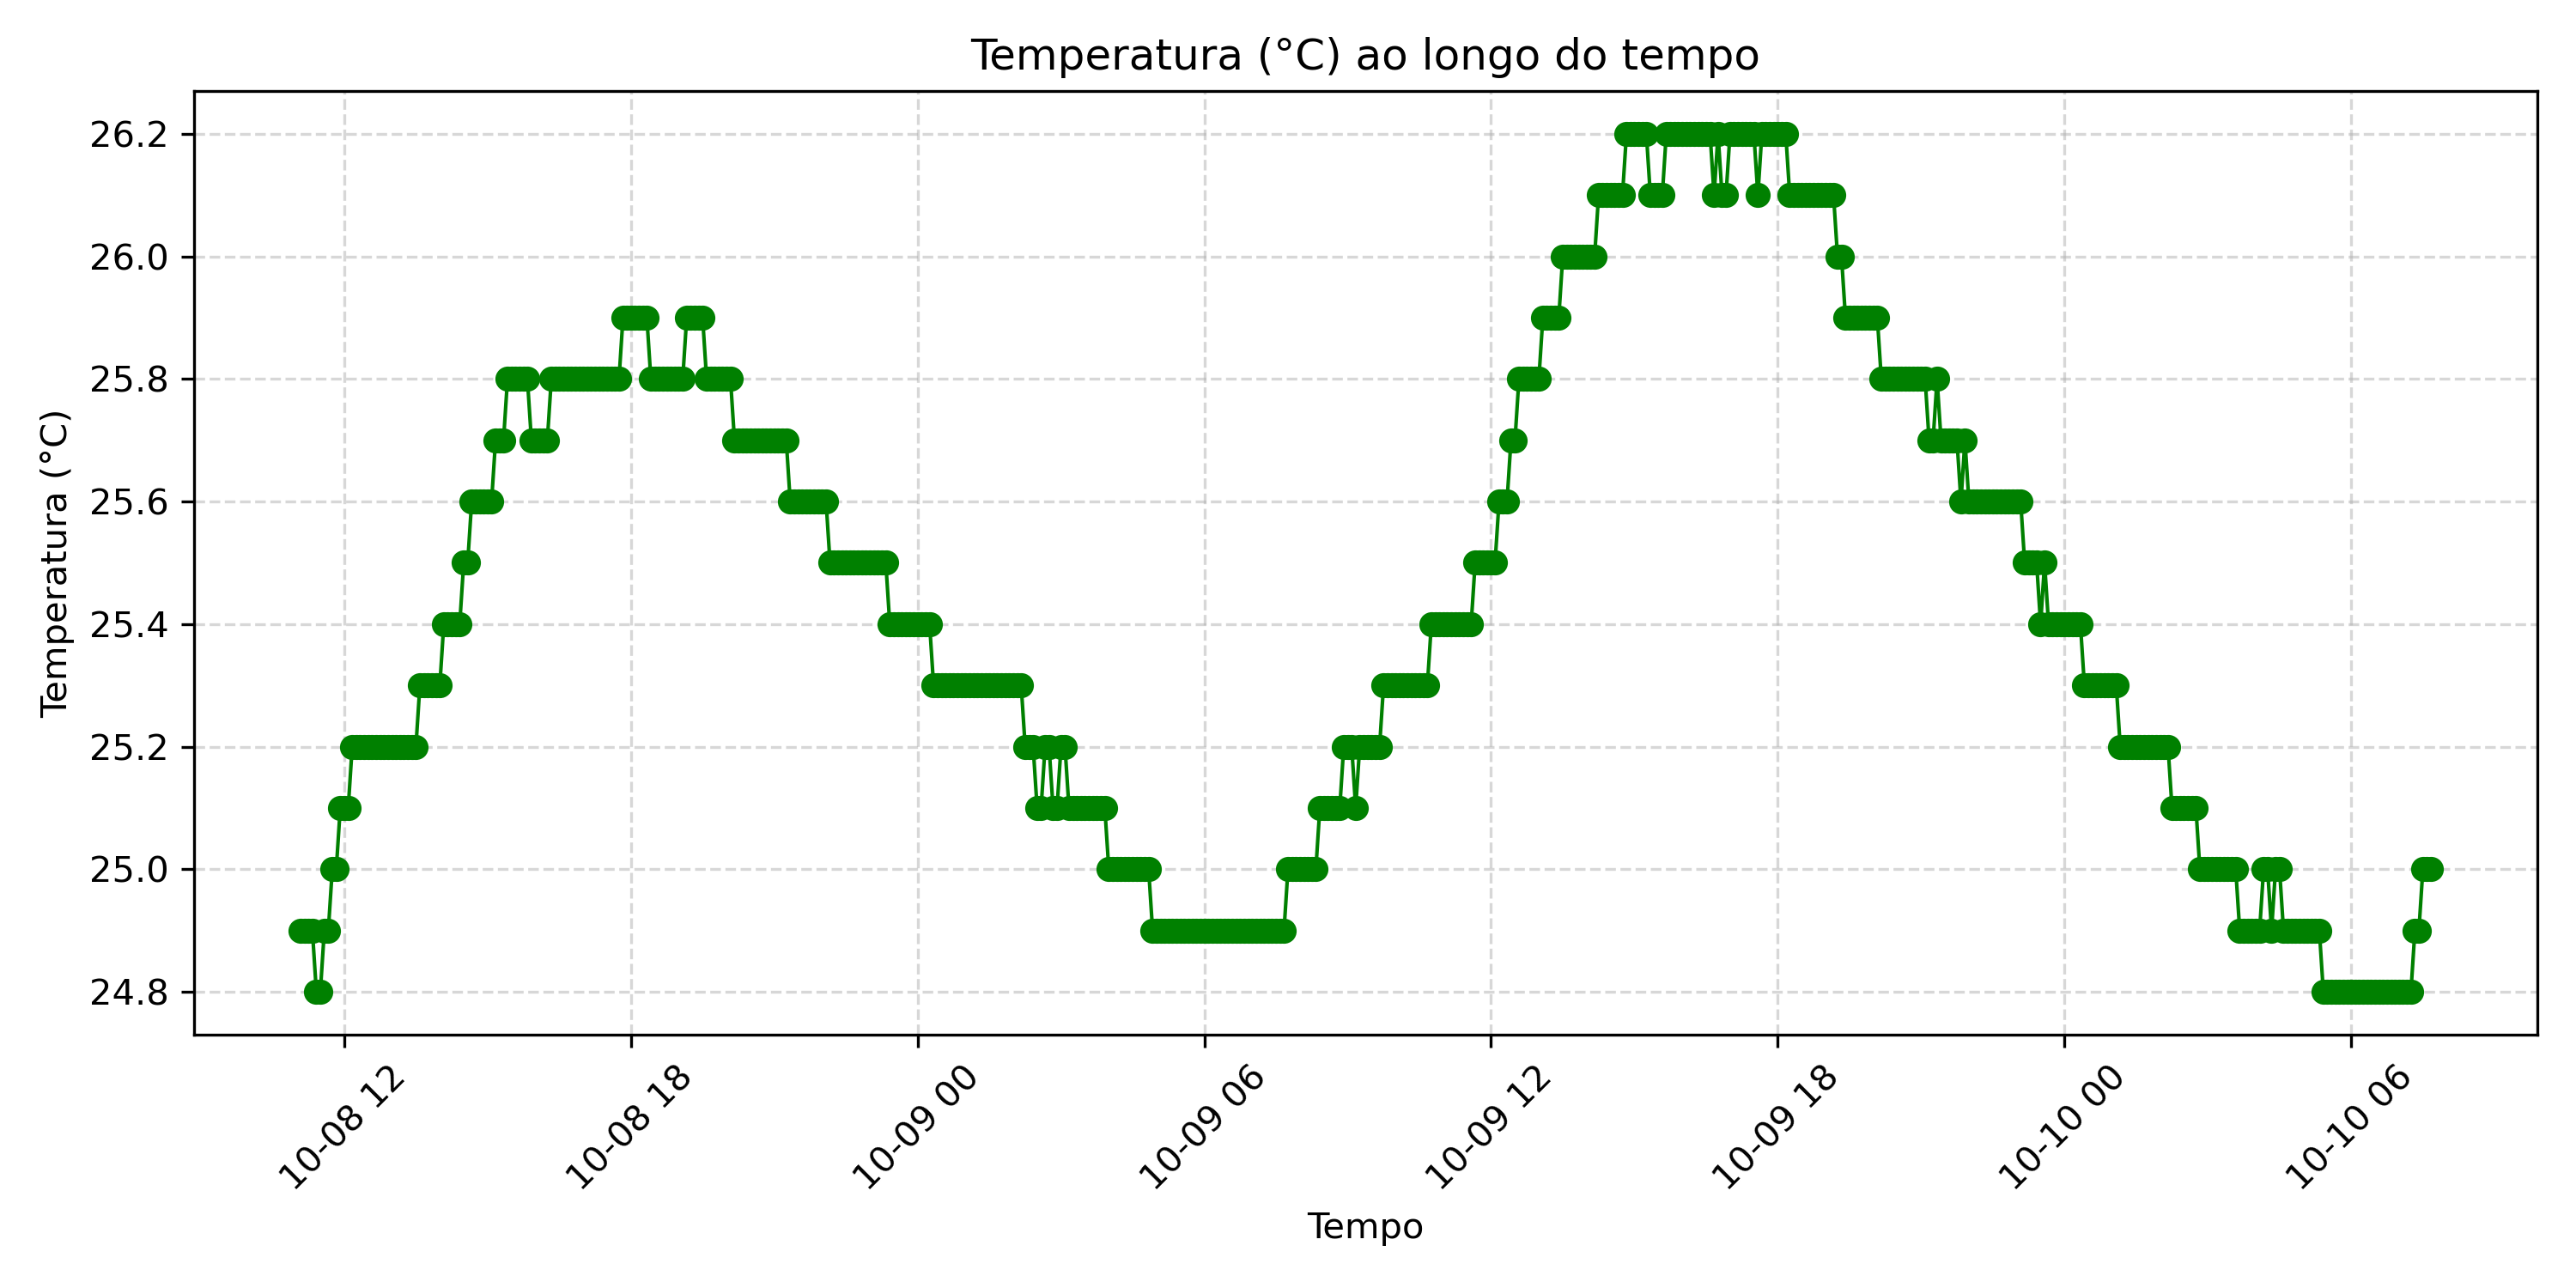
\includegraphics[width=0.8\textwidth]{Temp.png}
    \caption{Variação temporal da temperatura do ar}
\end{figure}
\end{frame}

\begin{frame}{Análise Estatística — Umidade do Ar}
\begin{itemize}
    \item Intervalo: \textbf{10,0\%};
    \item Média: \textbf{46,92\%};
    \item Mediana: \textbf{47,0\%};
    \item Desvio padrão: \textbf{1,70\%}.
\end{itemize}

\textbf{Conclusão:} Umidade do ar estável, ideal para hortaliças delicadas.

\begin{figure}[h]
    \centering
    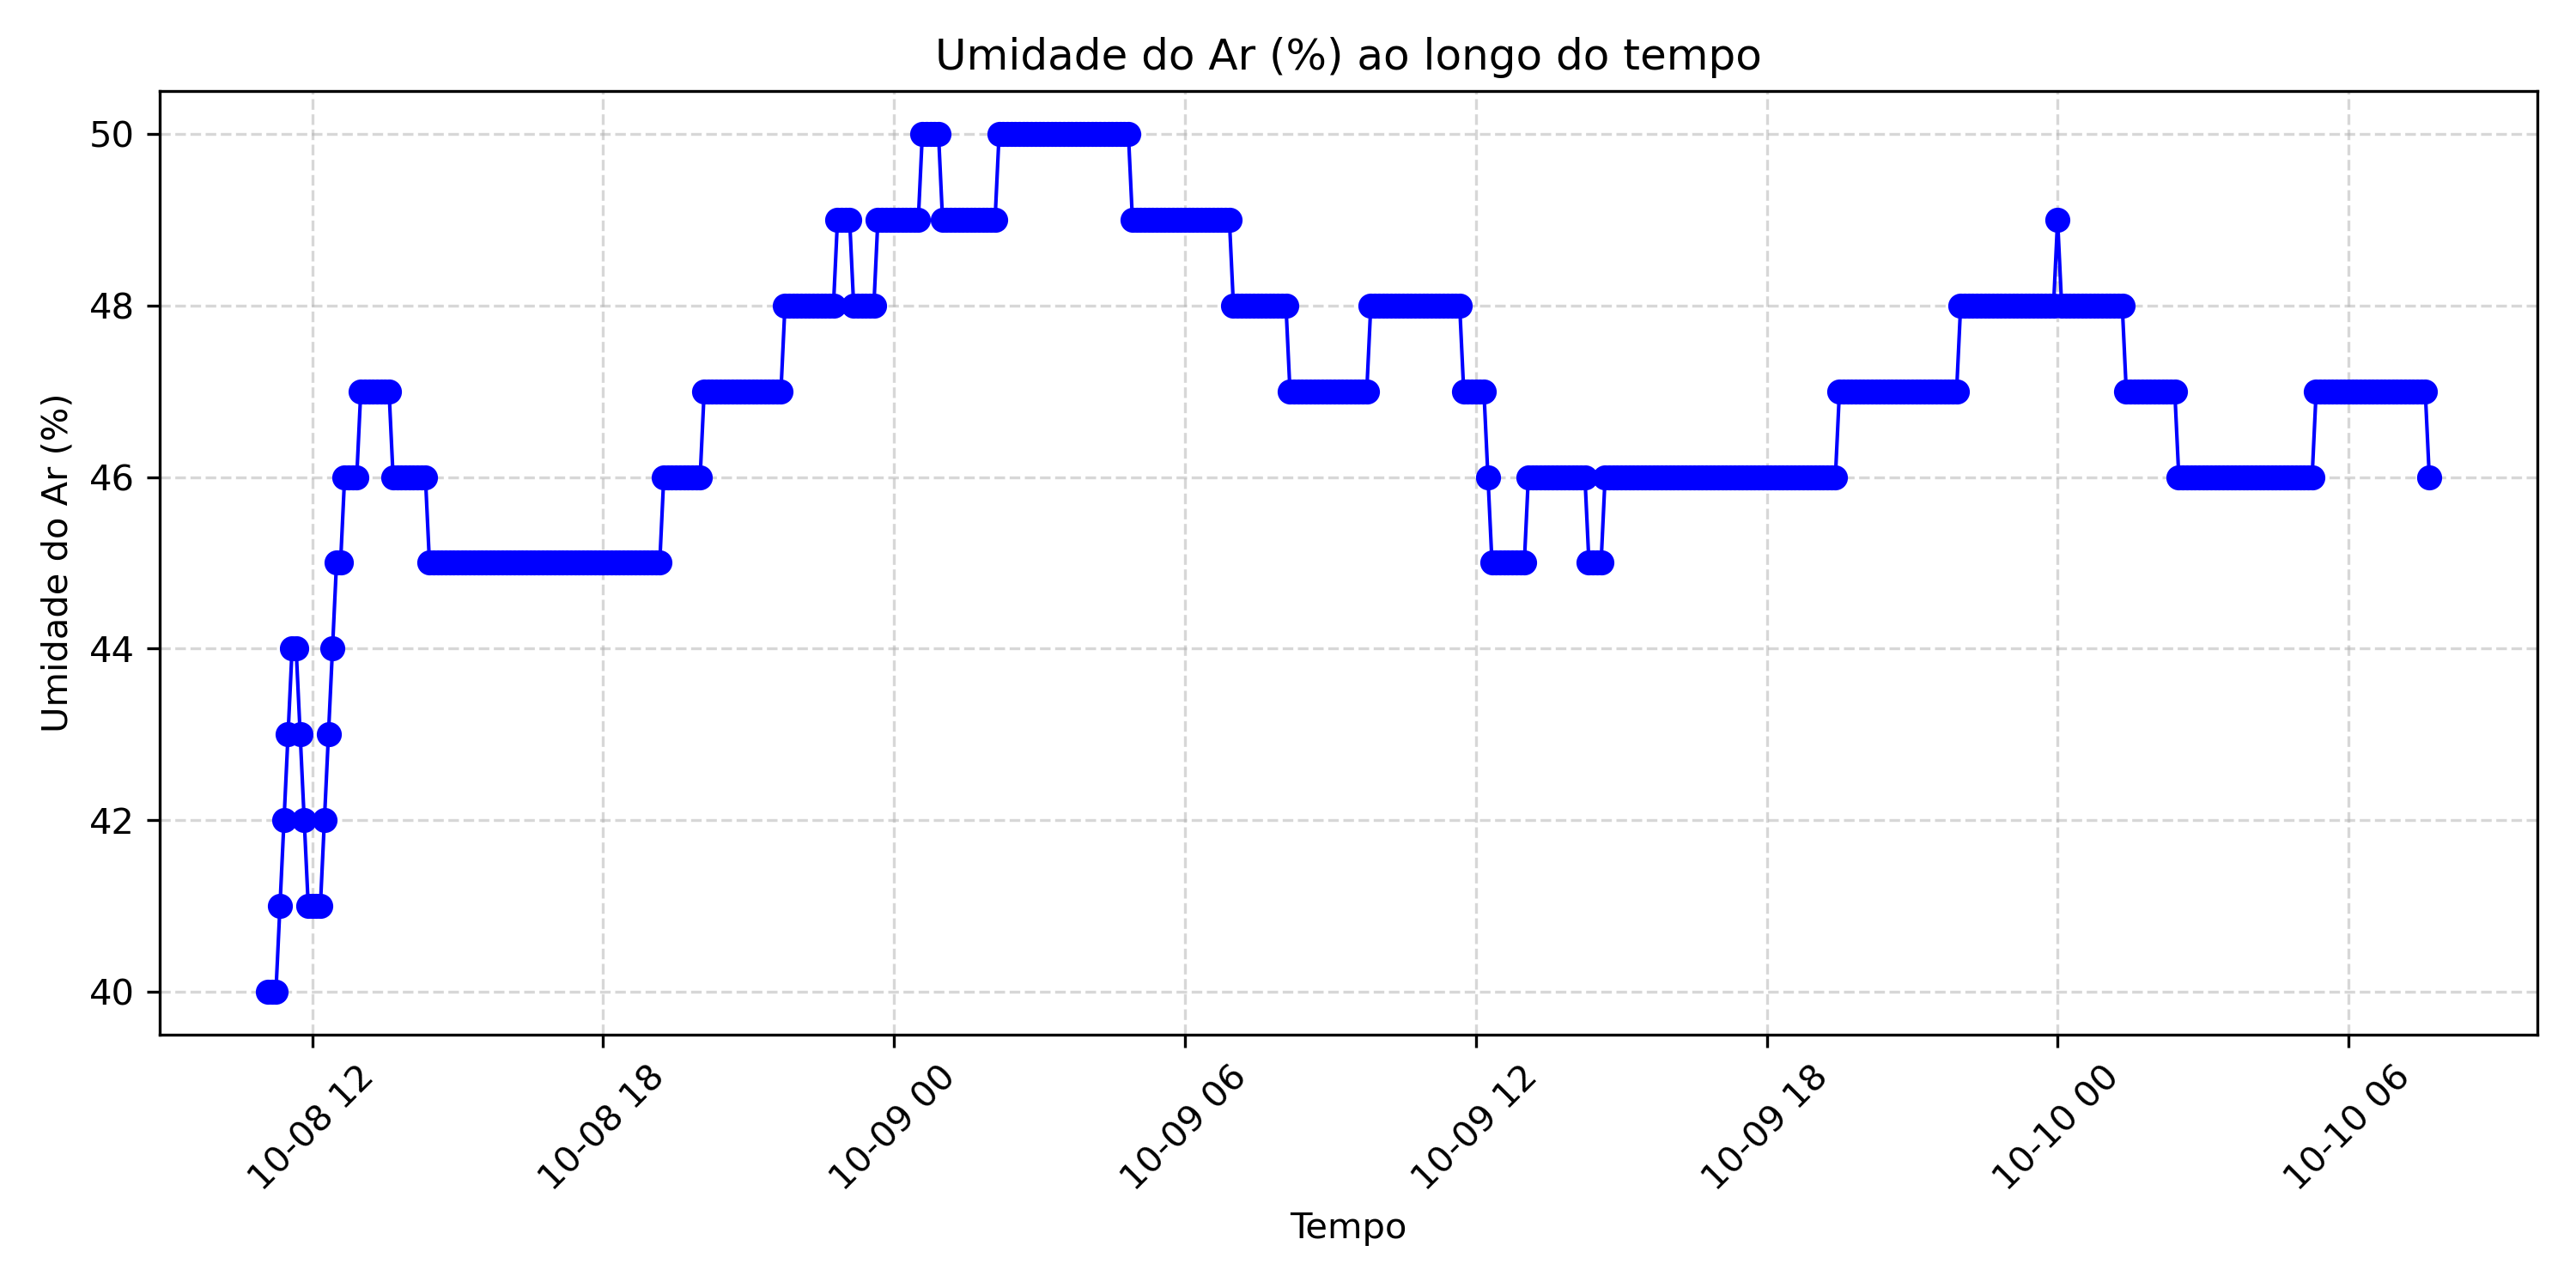
\includegraphics[width=0.8\textwidth]{UmidadeAr.png}
    \caption{Variação da umidade relativa do ar}
\end{figure}
\end{frame}

\begin{frame}{Análise Estatística — Umidade do Solo}
\begin{itemize}
    \item Intervalo: \textbf{31,0\%};
    \item Média: \textbf{80,39\%};
    \item Mediana: \textbf{82,0\%};
    \item Desvio padrão: \textbf{4,78\%}.
\end{itemize}

\textbf{Conclusão:} Solo com alta retenção hídrica, ideal para raízes e tubérculos.

\begin{figure}[h]
    \centering
    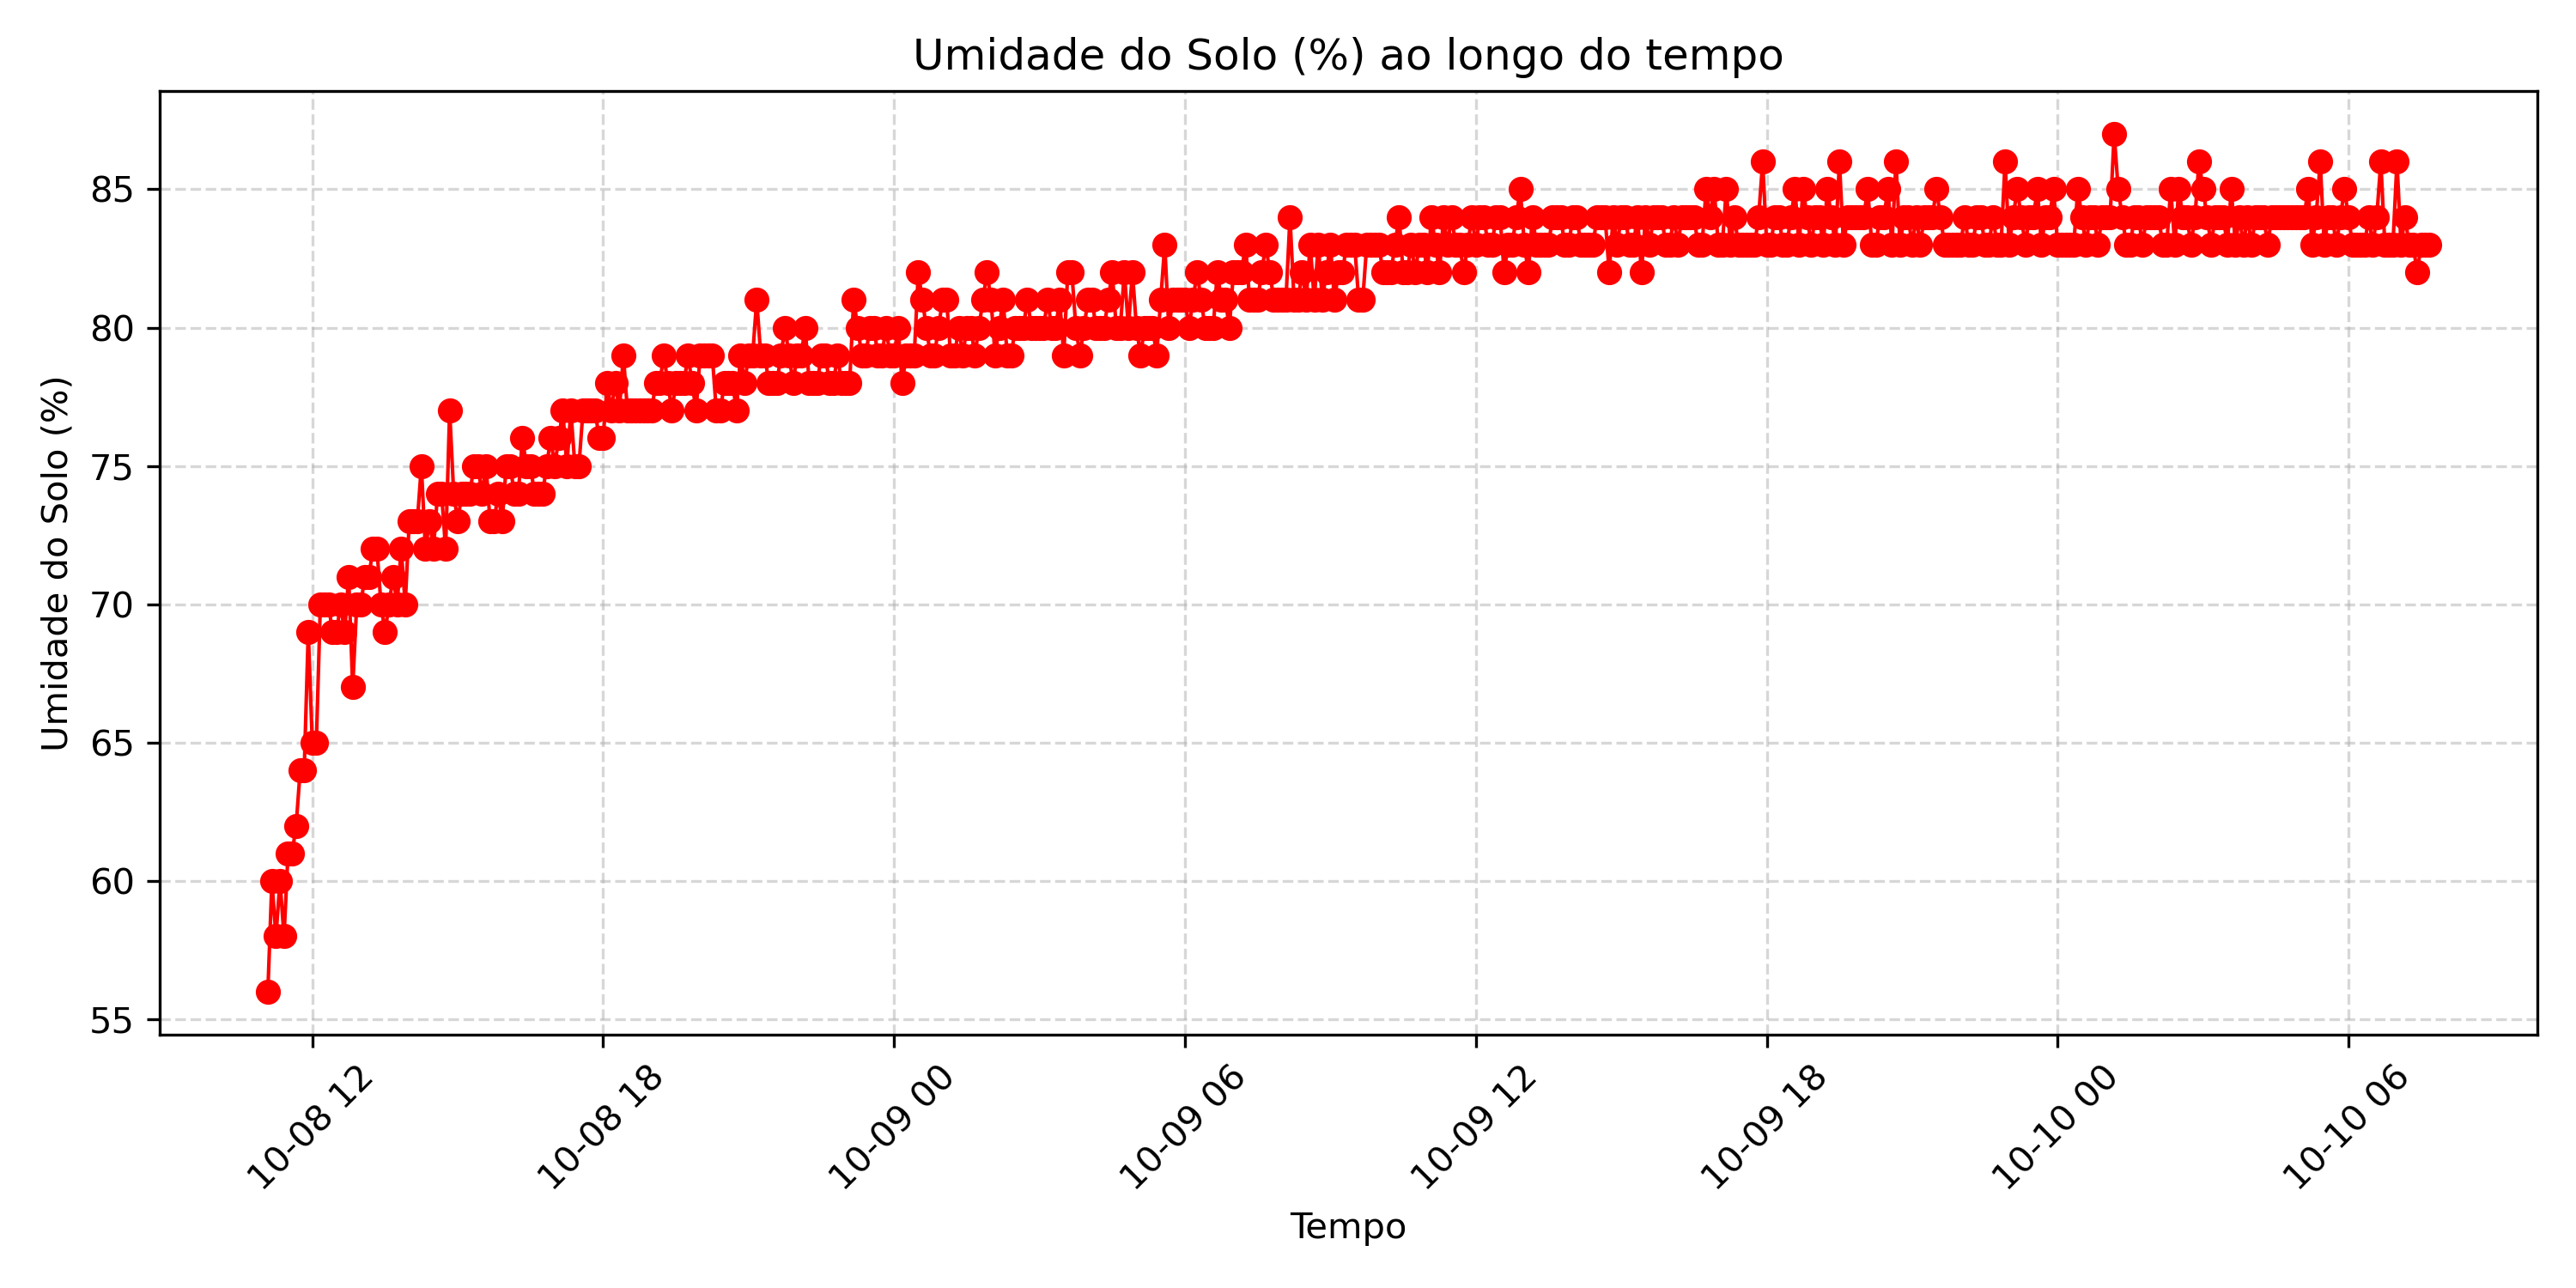
\includegraphics[width=0.8\textwidth]{USolo.png}
    \caption{Variação da umidade do solo}
\end{figure}
\end{frame}

% ==========================================================
% ====================== APRESENTADOR 3 ====================
% ==========================================================

\begin{frame}{Interpretação Agrícola}
\textbf{Culturas recomendadas:}
\begin{itemize}
    \item \textbf{Temperatura:} Tomate, feijão, pimentão;
    \item \textbf{Umidade do ar:} Alface, rúcula, hortelã;
    \item \textbf{Umidade do solo:} Cenoura, pepino, beterraba.
\end{itemize}

\textbf{Culturas não recomendadas:} Uva, lavanda e oliveira.
\end{frame}

\begin{frame}{Síntese Integrada}
\begin{itemize}
    \item O ambiente apresenta \textbf{alta estabilidade térmica} e \textbf{umidade elevada do solo}.
    \item Condições ideais para hortaliças e cultivos tropicais.
    \item O sistema permite controle inteligente de irrigação.
\end{itemize}

\begin{figure}[h]
    \centering
    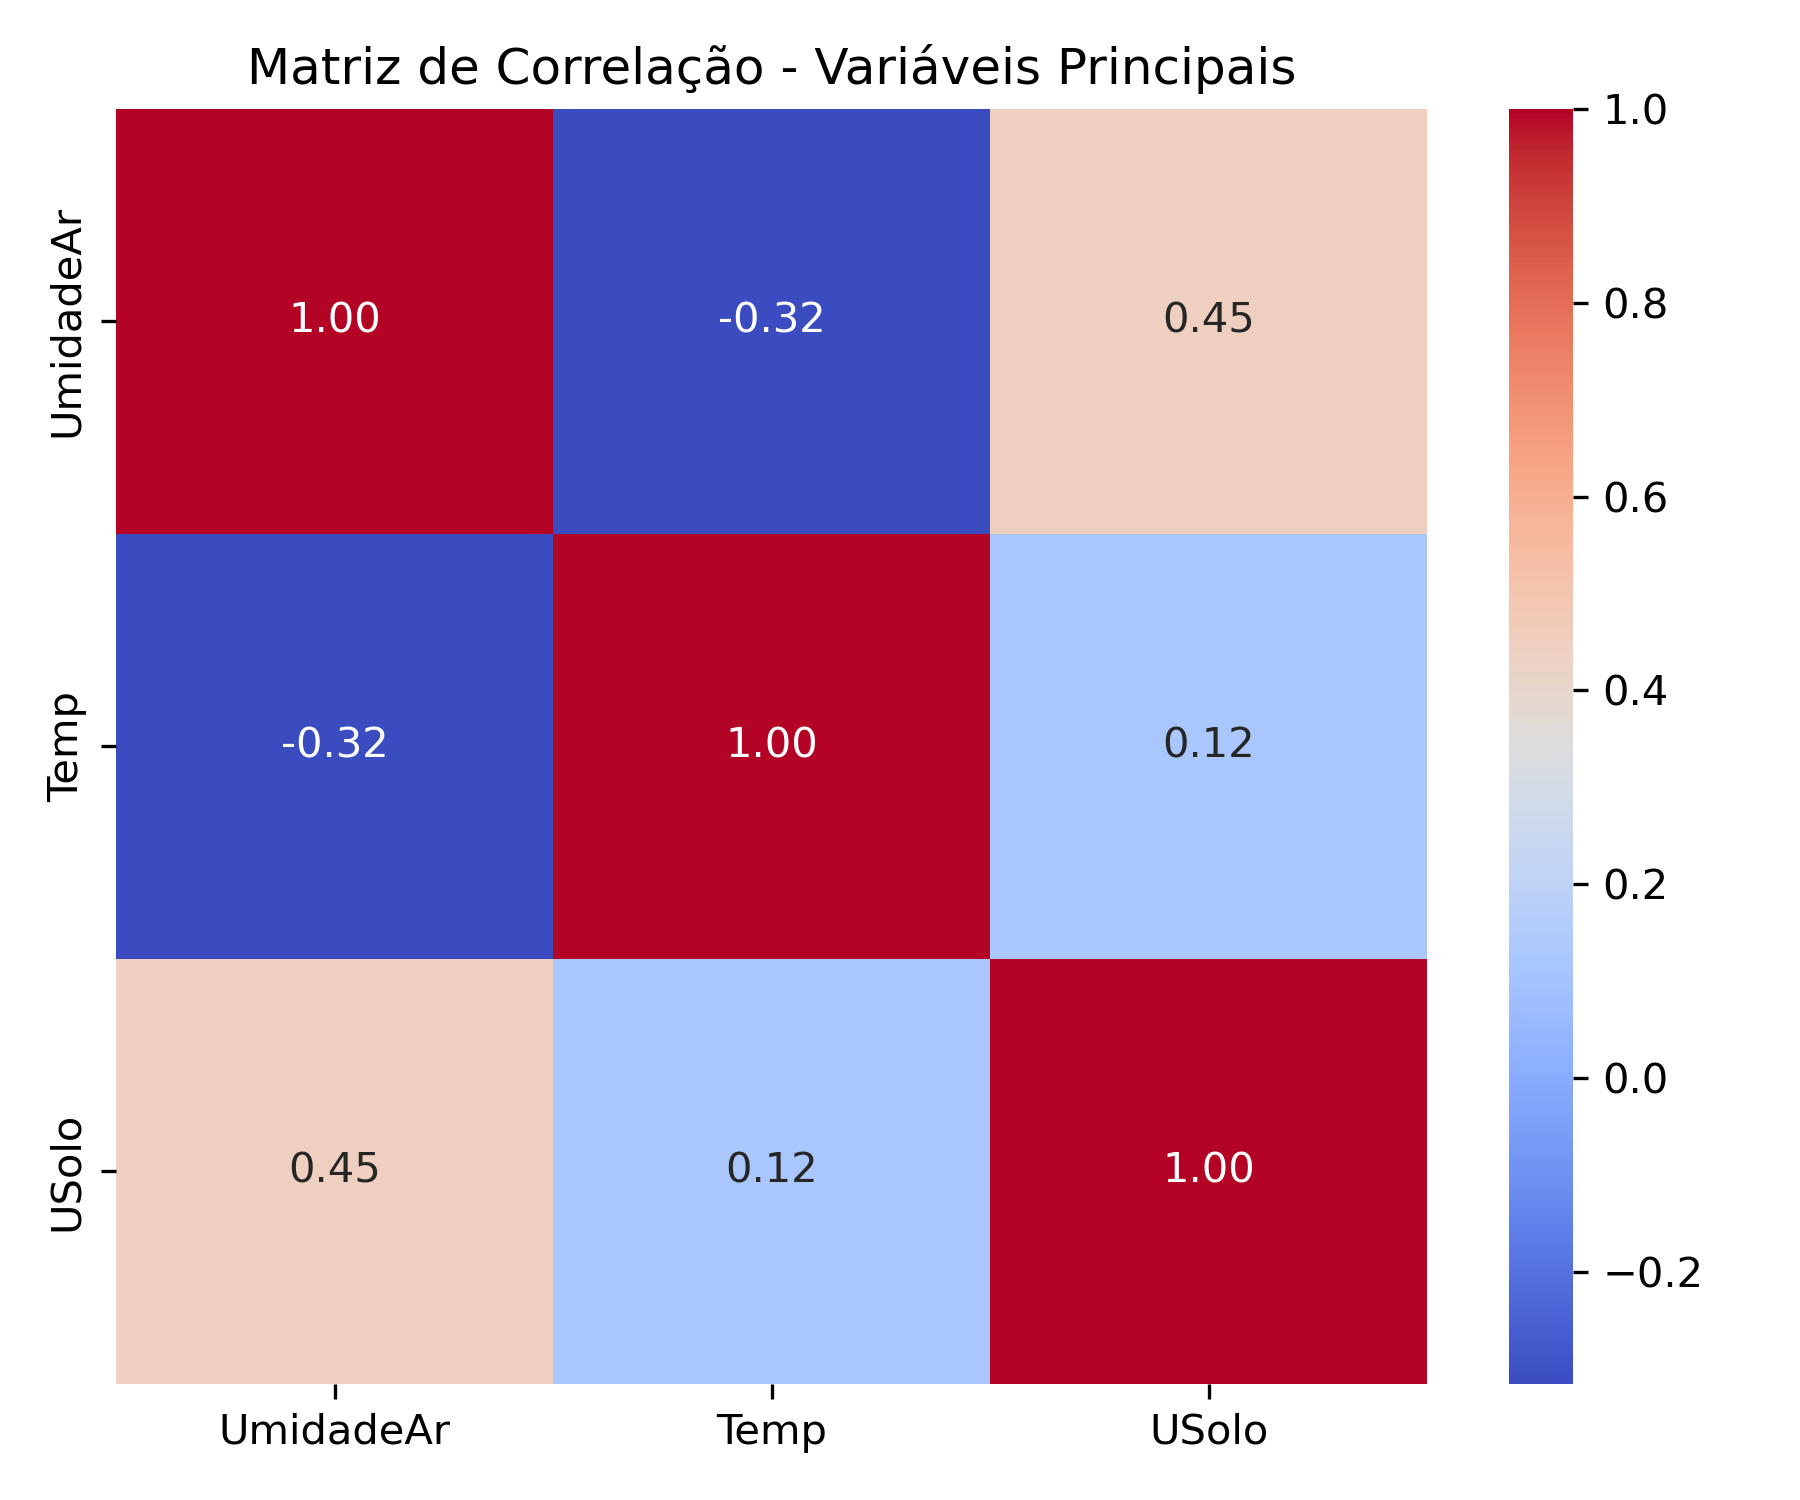
\includegraphics[width=0.8\textwidth]{correlacao_geral.png}
    \caption{Correlação entre variáveis ambientais}
\end{figure}
\end{frame}

\begin{frame}{Conclusão}
\begin{itemize}
    \item O sistema foi eficaz na coleta e análise dos dados ambientais.
    \item As condições indicam alto potencial produtivo e baixo risco climático.
    \item A integração entre eletrônica e estatística auxilia na agricultura sustentável.
\end{itemize}
\end{frame}

\end{document}

